Today, full compliance with all requirements can not be guaranteed. Thus, effective use of development methods and tools can reduce the probability for the occurrence of damage due to errors (software bugs) in a product.\\

In many products specific real-time operating systems (RTOSes) are used, which in comparison to universal OSes, having limited functionality, but much more predictable behaviour, which the key issue with real-time systems.\\

Despite the use of RTOSes, the temporal system behavior is difficult to predict, especially with high CPU loads. Thus, one approach is to utilize the processor(s) only 30 .. 50\%..\\

\os{\newpage}

{\rot\bf Host-Target Environment}\\

Embedded systems development usually takes place in host-target environments, mainly with a PC as a host on which the development environment is installed, and a binary file to download to the target system.Since with C programming language programming close-to-the-hardware is relatively simple and required, C dominates the embedded much more than any other programming language (but still, for computationally intensive algorithms assembly language is used). With applications using powerful computer systems, there are other programming languages, for example in avionics systems Ada is used.\\

\os{\newpage}

{\rot\bf Software Tests}\\

A software test is a test during software development to measure the functionality of a software to the requirements and their quality, and to identify software errors.

\nsl{\begin{enumerate}
\item  dynamic measures that require implementation of the software (e.g. test coverage)
\item  static measures that can do without an implementation of the software (e.g. code reviews)
\end{enumerate}}

There are several definitions for software testing:\\

ANSI/IEEE Std. 610.12-1990 defines test as the process of operating a system or component under specified conditions, observing or recording the results and making an evaluation of some aspects of the system or component.\\

Denert [1], defines test as "the verifiable and repeatable evidence of the correctness of a software building module relative to pre-established requirements".\\
\os{\newpage}

{\rot\bf Aim}

\begin{tcolorbox}[colback=blue!5!white,colframe=blue!75!black]
The aim of software testing is to detect errors !\\
But: to demonstrate that there are no errors, is not purpose of software testing !
\end{tcolorbox}

If in a test no errors are found, this never proves that the program is correct. The correctness of the program can't be proven by testing (except in trivial cases) !\\

The reason for this is that for a prove of correctness, all combinations of all possible values of the input data had to be tested: \\

A \textbf{simple realistic example:}\\

$\rightarrow$ 3 input variables, each 16 bit long leads to  \textit{N} = 2${}^{3.16}$ $\mathrm{\sim}$ 10${}^{16}$ possible combinations, with 1 s time for testing each combination, a complete test would take 8.9 Mio years. The number of combinations with real programs is too large for complete tests.\\

For this reason, different test strategies / concepts exist to deal with the question, how to achieve a maximum test coverage with the lowest possible number of test cases. \\

The results of software tests help to assess the true quality of the software.\\

{\rot\bf Test Planning}

\begin{enumerate}
\item  What requirements shall be tested in what depth ? 
\item  The number and the complexity of the test cases must be sufficient.
\item  Tests should be done at software development, ideally by the developers at  function/module level.
\end{enumerate}

The test design takes place in parallel to software development.\\

\os{\newpage}

{\rot\bf Requirements Engineering (RM)}

\begin{enumerate}
\item \textbf{ }The purpose of Requirements Management is to ensure that \textbf{\textit{complex products}} and \textbf{\textit{systems}} can be developed \textbf{\textit{in time}}, with the right \textbf{\textit{quality}}, at the right \textbf{\textit{costs}} !
\item  Requirements Management means, that \textbf{\textit{processes}} are defined and implemented for the tracing and documenting the complete development process: "intelligibility, clarity, traceability, consistency, completeness, testability". This \textbf{\textit{processes}} finally set the basis for defining the test cases !
\item  RM is well established in automotive industry  ISO/IEC 15504 (\textbf{\textit{SPICE}}). RM is closely connected to version- and configuration-management. RM is supported by database tools (e.g. \textbf{\textit{DOORS }(IBM/Rational)\textit{ }})
\end{enumerate}

\os{\newpage}

{\rot\bf V-Model of Testing}\\

    \begin{figure}[h]
    \centering
    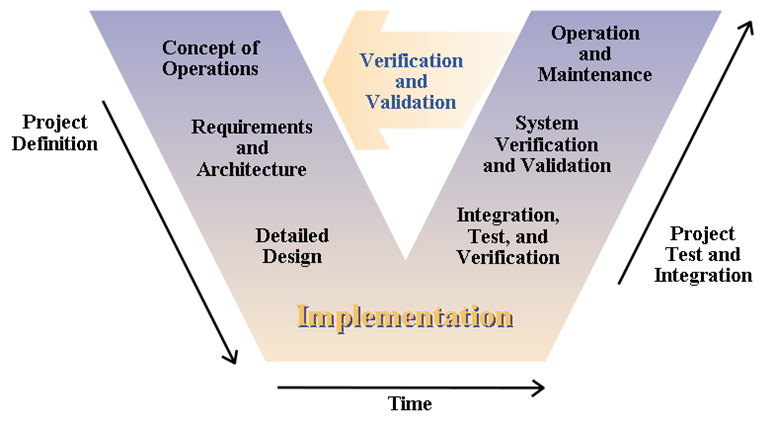
\includegraphics[width=12cm, height=6cm]{Images/image58.png}
    %\caption{}
    \label{fig:Fig 155}
    \end{figure}

\begin{itemize}
	\item The V-Model (or VEE model) of a systems engineering process.
	\item The classification of the test levels follows the timely progress of the project. In general, there are 4 test levels or test phases in the V-model.
\end{itemize}

\nsl{\begin{enumerate}
	\item  Unit test
	\item  Integration test 
	\item  System test 
	\item  Acceptance test
\end{enumerate}}

During development at each stage is tested against the corresponding specification.\\
\newpage

\textbf{1. Unit Test}\\

A unit test (component test) is a test on the deepest level. There, individual components are tested for proper functionality (hardware and software). Frequently, the software module test is carried out by the software developer, the test objects are single defined modules, functions or classes.\\

\textbf{2. Integration Test}\\

An integration test (or interaction test) tests the compliance of independent components. This can be hardware and software components, or integration of all tasks running with a common task schedule.\\

\textbf{3. System Test}\\

With a system test the whole system is tested against the total requirements (functional and non functional requirements tested). Usually the test is done with automatic test environment using test data to simulate the final environment (e.g. squeeze force tests with a door ECU with a software anti-squeeze function).\\

\textbf{ 4. Acceptance Test}\\

An acceptance test, or user acceptance test (UAT) is a test of the product by the customer. Often, acceptance tests are required for billing. \\
In an acceptance test, the black-box method is used, i.e. the customer does not consider the code of the software, but only the behavior of the software at specified actions E.g.: the ECU with anti-squeeze software is tested with a door

\begin{enumerate}
\item  environmental tests with the complete temperature range (-40$\mathrm{{}^\circ}$ to 95$\mathrm{{}^\circ}$)
\item  various noise on supply conditions (like pulses)
\item  different test objects
\end{enumerate}

\os{\newpage}
{\rot\bf Test Automation}\\

Particularly, tests that need to be repeated often, test automation is advisable, if aor test to be done manually is not feasible, difficult, or too expensive (e.g. lifetime tests).
Test automation is also especially useful for regression testing. 

\begin{enumerate}
\item  Regression Testing is used after software changes to assure already achieved functionality.
\end{enumerate}

    \begin{figure}[h]
    \centering
    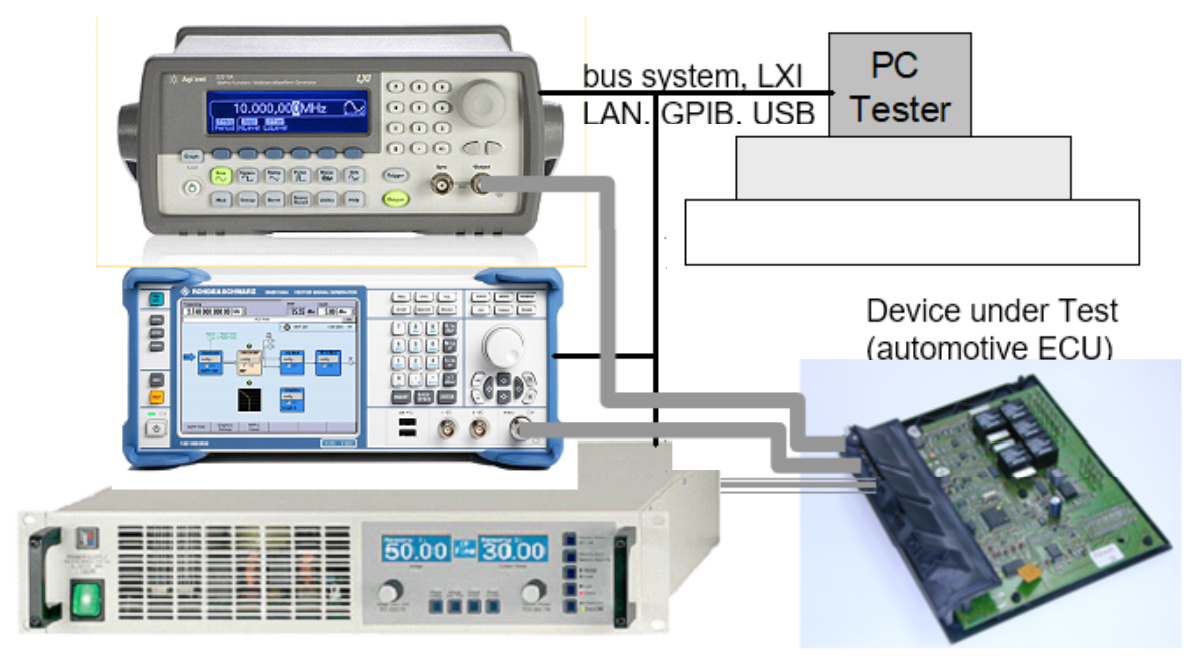
\includegraphics[width=15cm, height=8cm]{Images/image182.png}
    %\caption{}
    \label{fig:Fig 156}
    \end{figure}

\textbf{PC-Software:}

 \begin{enumerate}
	\item  LabWindows, LabView, C, C\#, VisualBasic
	\item  MATLAB + Data Acquisition Toolbox
	\item  DSpace
	\item  VISA (Python + VISA, OpenSource)
\end{enumerate}






